% Options for packages loaded elsewhere
\PassOptionsToPackage{unicode}{hyperref}
\PassOptionsToPackage{hyphens}{url}
%
\documentclass[
  x11names]{article}
\usepackage{amsmath,amssymb}
\usepackage{lmodern}
\usepackage{iftex}
\ifPDFTeX
  \usepackage[T1]{fontenc}
  \usepackage[utf8]{inputenc}
  \usepackage{textcomp} % provide euro and other symbols
\else % if luatex or xetex
  \usepackage{unicode-math}
  \defaultfontfeatures{Scale=MatchLowercase}
  \defaultfontfeatures[\rmfamily]{Ligatures=TeX,Scale=1}
\fi
% Use upquote if available, for straight quotes in verbatim environments
\IfFileExists{upquote.sty}{\usepackage{upquote}}{}
\IfFileExists{microtype.sty}{% use microtype if available
  \usepackage[]{microtype}
  \UseMicrotypeSet[protrusion]{basicmath} % disable protrusion for tt fonts
}{}
\makeatletter
\@ifundefined{KOMAClassName}{% if non-KOMA class
  \IfFileExists{parskip.sty}{%
    \usepackage{parskip}
  }{% else
    \setlength{\parindent}{0pt}
    \setlength{\parskip}{6pt plus 2pt minus 1pt}}
}{% if KOMA class
  \KOMAoptions{parskip=half}}
\makeatother
\usepackage{xcolor}
\usepackage[margin=1in]{geometry}
\usepackage{graphicx}
\makeatletter
\def\maxwidth{\ifdim\Gin@nat@width>\linewidth\linewidth\else\Gin@nat@width\fi}
\def\maxheight{\ifdim\Gin@nat@height>\textheight\textheight\else\Gin@nat@height\fi}
\makeatother
% Scale images if necessary, so that they will not overflow the page
% margins by default, and it is still possible to overwrite the defaults
% using explicit options in \includegraphics[width, height, ...]{}
\setkeys{Gin}{width=\maxwidth,height=\maxheight,keepaspectratio}
% Set default figure placement to htbp
\makeatletter
\def\fps@figure{htbp}
\makeatother
\setlength{\emergencystretch}{3em} % prevent overfull lines
\providecommand{\tightlist}{%
  \setlength{\itemsep}{0pt}\setlength{\parskip}{0pt}}
\setcounter{secnumdepth}{-\maxdimen} % remove section numbering
\usepackage{fontspec} \usepackage{titling} \usepackage{framed} \pretitle{\begin{center} \vspace{-3cm}
\includegraphics[width=\linewidth]{images/Base_info/logo.png}\LARGE\\} \posttitle{\end{center}} \usepackage{float} \usepackage{fancyhdr} \usepackage{ragged2e} \usepackage{caption} \usepackage{colortbl} \captionsetup[figure]{labelformat=empty} \arrayrulecolor{white} \pagestyle{fancy} \fancyhead[L,C]{} \fancypagestyle{plain}{\pagestyle{fancy}} \PassOptionsToPackage{dvipsnames,svgnames*,x11names*}{xcolor} \definecolor{ceil}{rgb}{0.57, 0.63, 0.81} \usepackage[export]{adjustbox} \usepackage{wrapfig} \usepackage{graphicx} \usepackage{caption}
\usepackage{booktabs}
\usepackage{longtable}
\usepackage{array}
\usepackage{multirow}
\usepackage{wrapfig}
\usepackage{float}
\usepackage{colortbl}
\usepackage{pdflscape}
\usepackage{tabu}
\usepackage{threeparttable}
\usepackage{threeparttablex}
\usepackage[normalem]{ulem}
\usepackage{makecell}
\usepackage{xcolor}
\ifLuaTeX
  \usepackage{selnolig}  % disable illegal ligatures
\fi
\IfFileExists{bookmark.sty}{\usepackage{bookmark}}{\usepackage{hyperref}}
\IfFileExists{xurl.sty}{\usepackage{xurl}}{} % add URL line breaks if available
\urlstyle{same} % disable monospaced font for URLs
\hypersetup{
  hidelinks,
  pdfcreator={LaTeX via pandoc}}

\author{}
\date{\vspace{-2.5em}Fecha de creación: 06 April, 2023}

\begin{document}

\renewenvironment{framed}[1][\hsize]
  {\MakeFramed{\hsize#1\advance\hsize-\width \FrameRestore}}%
  {\endMakeFramed}

\setmainfont{Arial}
\setsansfont{Arial}
\setmonofont{Arial}

\newcommand\invisiblesection[1]{%
  \refstepcounter{section}%
  \addcontentsline{toc}{section}{\protect\numberline{\thesection}#1}%
  \sectionmark{#1}}

\fancyhead[R]{\textbf{http://doi.org/10.31687/SaremLR.19.150}}

%
  \refstepcounter{section}%
  \addcontentsline{toc}{section}{\protect\numberline{\thesection}GENERALIDADES}%
  \sectionmark{GENERALIDADES}
\vspace{-0.4cm}


\includegraphics[width=1\linewidth]{images/Base_info/logo}

\vspace{1cm}

\begin{minipage}{0.7\textwidth}
\vspace{0.3cm}
\fontsize{20}{24}\selectfont\textit{Puma concolor}

\vspace{0.3cm}
\fontsize{30}{36}\selectfont Puma
\end{minipage}
\hspace{0.05\textwidth}
\begin{minipage}{0.25\textwidth}

\includegraphics[width=\textwidth]{images/lc.png}
\end{minipage}

\normalsize

\begin{figure}[H]

{\centering 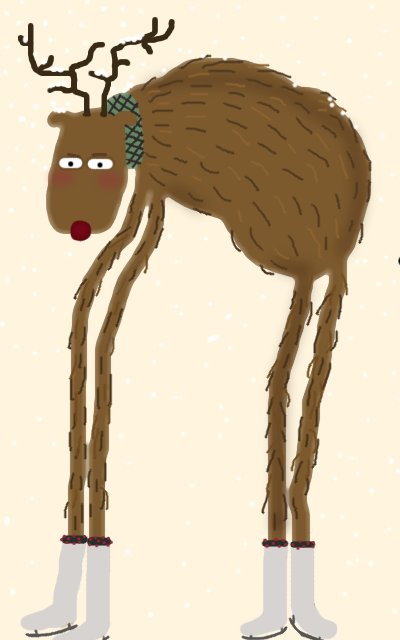
\includegraphics[width=0.35\linewidth]{photos/Blastocerus dichotomus} 

}

\caption{Fotos por Salvador Dali}\label{fig:image}
\end{figure}

\begin{center}\rule{0.5\linewidth}{0.5pt}\end{center}

\justifying

\textbf{Citar como:} De Angelo, Carlos; Llanos, Romina; Guerisoli, María
de las Mercedes; Varela, Diego; Valenzuela, Alejandro E. J.; Pía, Mónica
V.; Monteverde, Martín; Reppucci, Juan I.; Lucherini, Mauro; D'Agostino,
Romina; Bolgeri, María José; Quiroga, Verónica A.. (2019). \emph{Puma
concolor}. En: SAyDS--SAREM (eds.) Categorización 2019 de los mamíferos
de Argentina según su riesgo de extinción. Lista Roja de los mamíferos
de Argentina. \url{http://doi.org/10.31687/SaremLR.19.150}

\begin{center}\rule{0.5\linewidth}{0.5pt}\end{center}

\newpage

%
  \refstepcounter{section}%
  \addcontentsline{toc}{section}{\protect\numberline{\thesection}ÁREA DE DISTRIBUCIÓN ACTUAL}%
  \sectionmark{ÁREA DE DISTRIBUCIÓN ACTUAL}
\begin{table}[H]
\centering
\begin{tabular}[t]{>{\raggedright\arraybackslash}m{16cm}>{}m{16cm}}
\toprule
\cellcolor{ceil}{\textcolor{white}{\textbf{\rule{0pt}{14pt}ÁREA DE DISTRIBUCIÓN ACTUAL}}}\\
\bottomrule
\end{tabular}
\end{table}

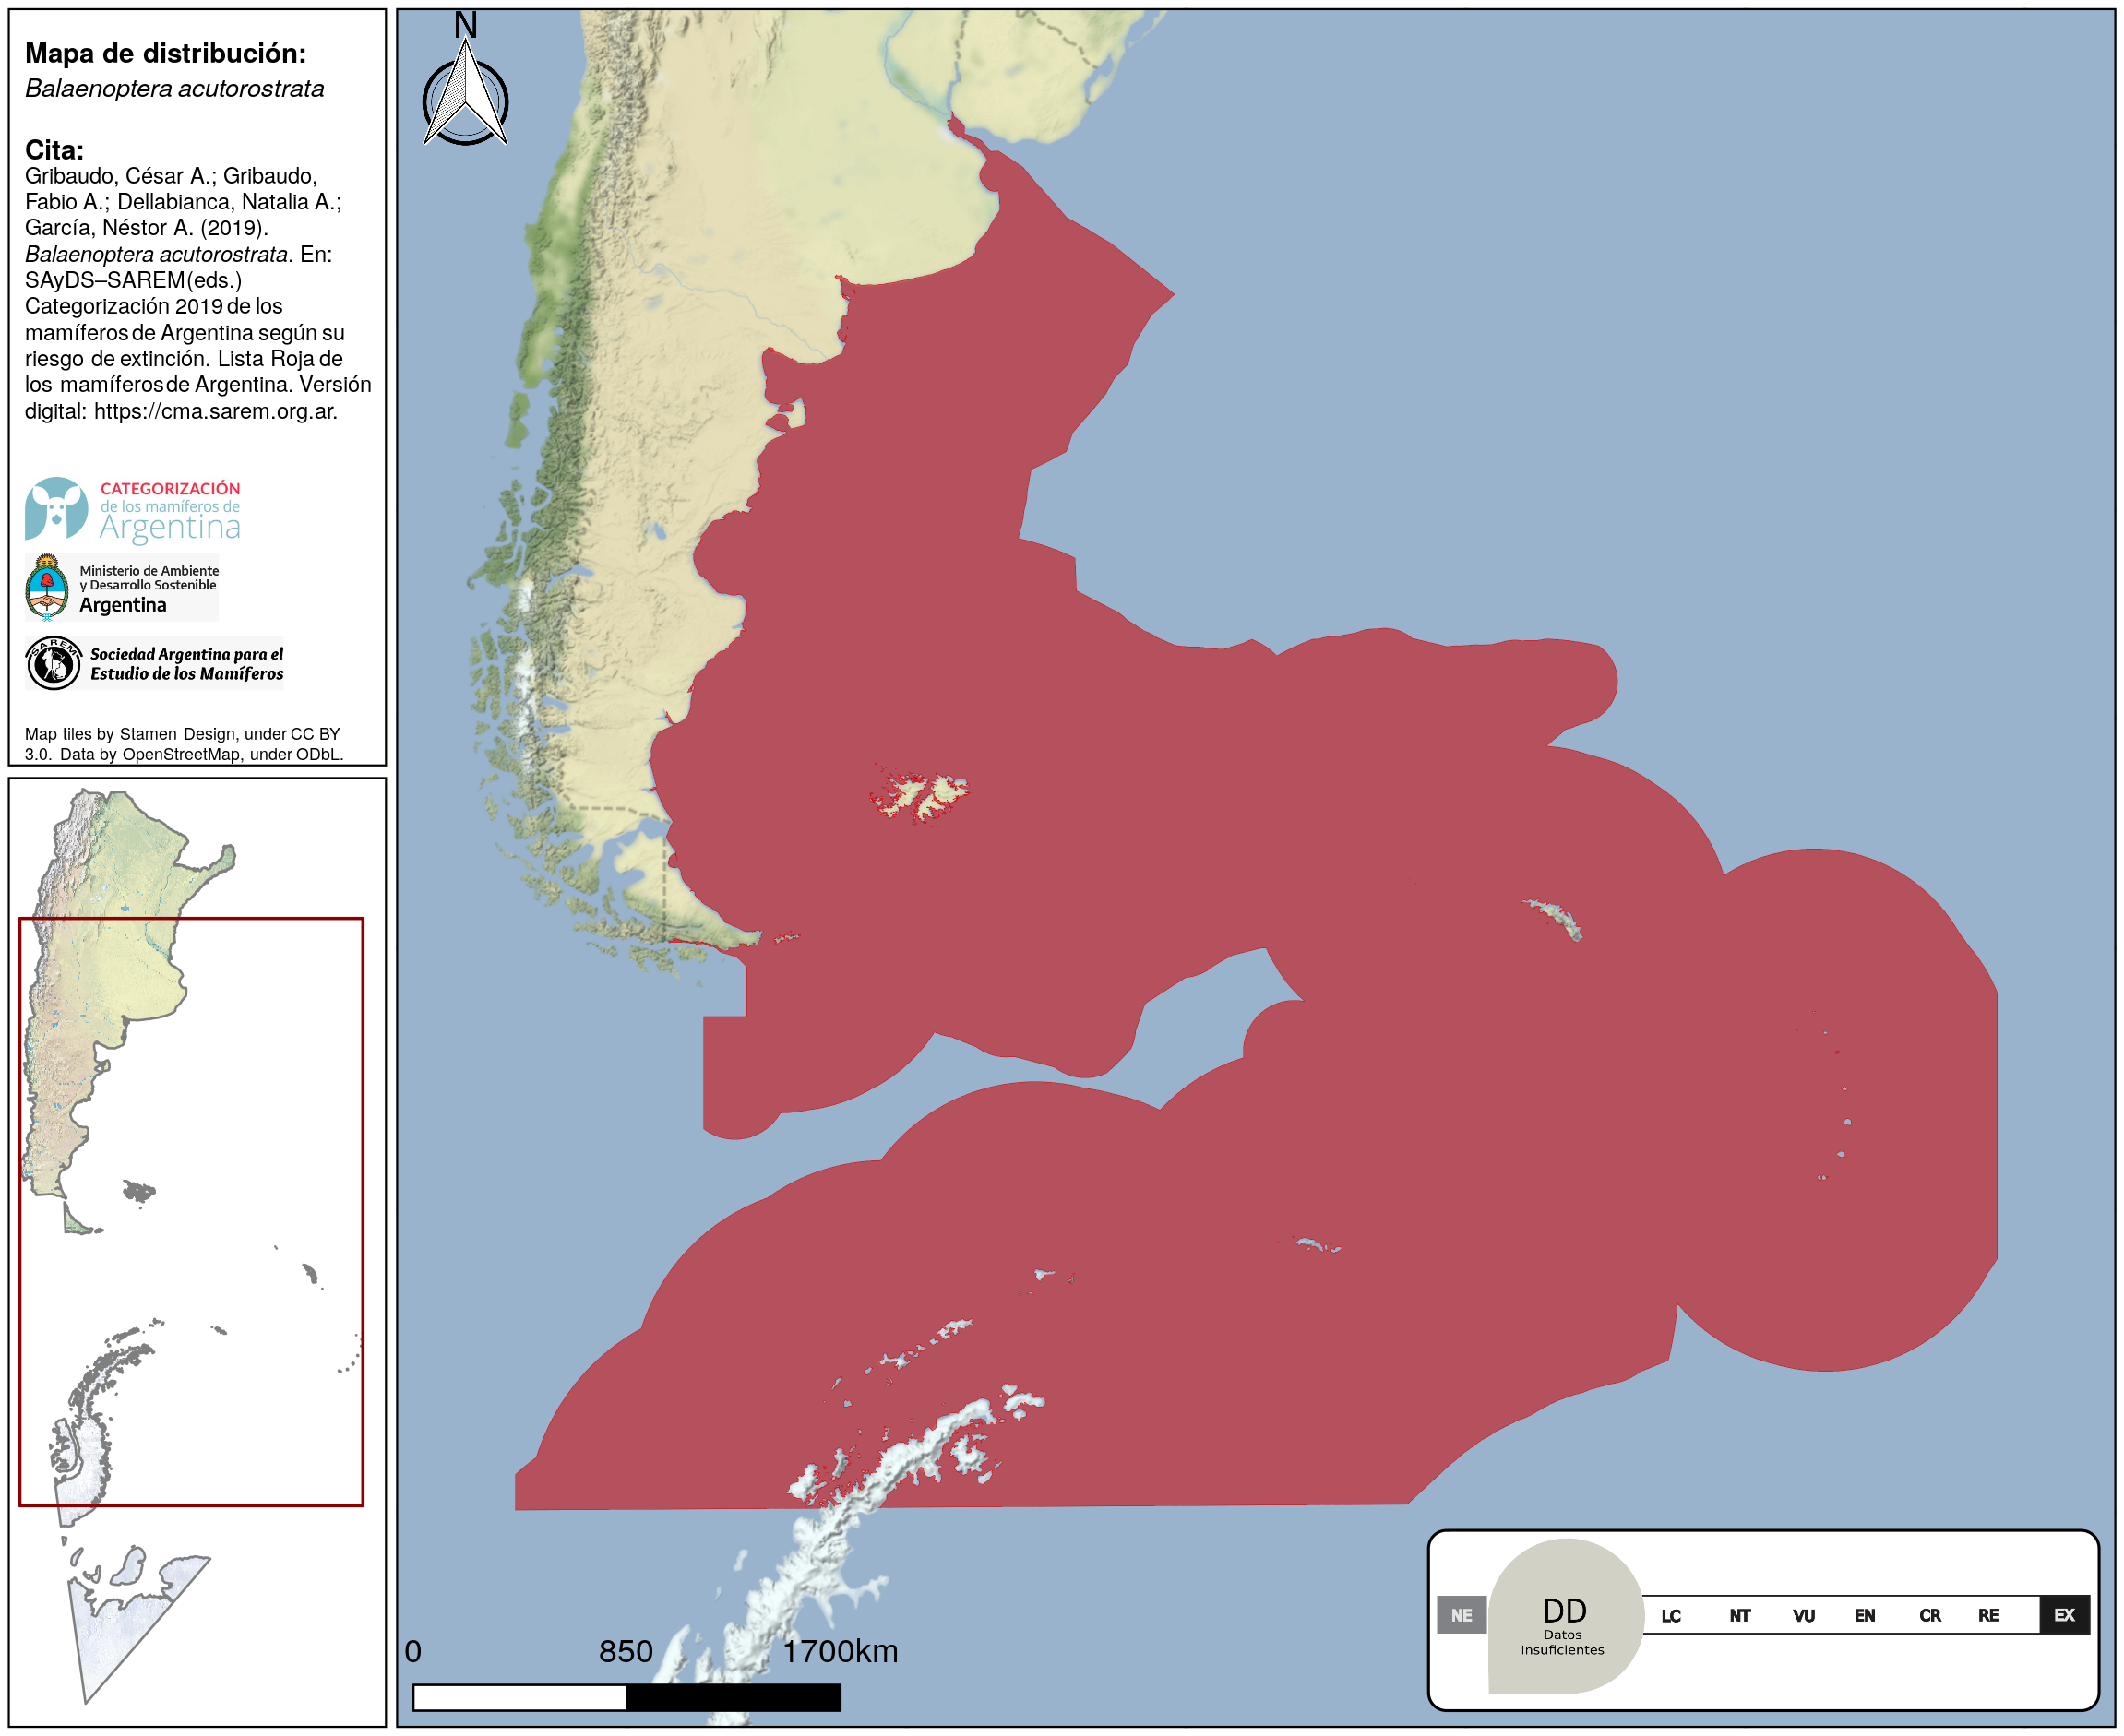
\includegraphics[width=1\linewidth]{maps/Cetartiodactyla/Balaenoptera_acutorostrata}

%
  \refstepcounter{section}%
  \addcontentsline{toc}{section}{\protect\numberline{\thesection}CATEGORÍAS DE CONSERVACIÓN}%
  \sectionmark{CATEGORÍAS DE CONSERVACIÓN}
\begin{table}[H]
\centering
\begin{tabular}[t]{>{\raggedright\arraybackslash}m{16cm}>{}m{16cm}}
\toprule
\cellcolor{ceil}{\textcolor{white}{\textbf{\rule{0pt}{14pt}CATEGORÍAS DE CONSERVACIÓN}}}\\
\bottomrule
\end{tabular}
\end{table}

\vspace{-0.4cm}

\textbf{Categoría Nacional de Conservación 2019}

LC (Preocupación Menor)

\textbf{Criterios y subcriterios}

NA

\textbf{Justificación de la categorización}

Es una especie generalista, que habita gran parte del territorio
nacional, incluyendo áreas altamente modificadas por el hombre. Como se
mencionó en la recategorización previa (Aprile et al.~2012), localmente
el puma puede estar sufriendo retracciones puntuales en algunas regiones
producto de la persecución directa y la expansión de la frontera
agropecuaria. Sin embargo, esta retracción difícilmente superaría el
30\% del área actual de la especie en el país en 3 generaciones, sobre
todo si consideramos que habita en ambientes muy modificados y que ha
demostrado una alta capacidad de recuperación y repoblamiento en algunos
sectores. La EOO estimada para la especie es ampliamente superior a los
20.000 km2 (más de 3 millones de km2). Debido a esta amplia distribución
y demás factores mencionados, y a que sus poblaciones son continuas con
las de países vecinos, se sugiere mantener la categorización del puma
como Preocupación Menor (LC) en la Argentina. No obstante, se enfatiza
su importante rol ecológico como depredador tope y se sostiene la
recomendación de monitorear algunas de sus sub-poblaciones que se
perciban bajo amenaza, ya que pueden estar en riesgo por la persecución
directa de la especie o la modificación del hábitat, y llegar a
desaparecer como ha ocurrido en muchas regiones durante el siglo XX.

\textbf{Categoría Res. SAyDS 1030/04}

NA (No Amenazada)

\textbf{Categorías nacionales de conservación previas (SAREM)}

\begin{tabu} to \linewidth {>{}l>{\raggedright}X>{\raggedright}X}
\toprule
\textbf{\cellcolor{gray!6}{2012}} & \cellcolor{gray!6}{LC (Preocupación Menor)} & \cellcolor{gray!6}{NA}\\
\bottomrule
\end{tabu}

\begin{tabu} to \linewidth {>{}l>{\raggedright}X>{\raggedright}X}
\toprule
\textbf{\cellcolor{gray!6}{2000}} & \cellcolor{gray!6}{LR nt (Riesgo Bajo, potencialmente vulnerable)} & \cellcolor{gray!6}{NA}\\
\bottomrule
\end{tabu}

\begin{tabu} to \linewidth {>{}l>{\raggedright}X>{\raggedright}X}
\toprule
\textbf{\cellcolor{gray!6}{1997}} & \cellcolor{gray!6}{RB pm (Riesgo Bajo, preocupación menor; LR lc)} & \cellcolor{gray!6}{NA}\\
\bottomrule
\end{tabu}

\begin{tabu} to \linewidth {>{}l>{\raggedright}X}
\toprule
\textbf{\cellcolor{gray!6}{Homologación categoría 1997}} & \cellcolor{gray!6}{LC (Preocupación Menor)}\\
\bottomrule
\end{tabu}

\textbf{Categorías de conservación actuales en países vecinos}

\begin{tabu} to \linewidth {>{\raggedright}X>{\raggedright}X>{\raggedright}X>{\raggedright}X}
\toprule
\textbf{País} & \textbf{Categoría} & \textbf{Año} & \textbf{Cita}\\
\arrayrulecolor{white}
\midrule
\cellcolor{gray!6}{Bolivia} & \cellcolor{gray!6}{LC (Preocupación Menor)} & \cellcolor{gray!6}{2009} & \cellcolor{gray!6}{Tarifa \&amp; Aguirre (2009)}\\
\bottomrule
\end{tabu}
\begin{tabu} to \linewidth {>{\raggedright}X>{\raggedright}X>{\raggedright}X>{\raggedright}X}
\toprule
\textbf{País} & \textbf{Categoría} & \textbf{Año} & \textbf{Cita}\\
\arrayrulecolor{white}
\midrule
\cellcolor{gray!6}{Brasil} & \cellcolor{gray!6}{VU (Vulnerable)} & \cellcolor{gray!6}{2013} & \cellcolor{gray!6}{de Azevedo et al. (2013)}\\
\bottomrule
\end{tabu}
\begin{tabu} to \linewidth {>{\raggedright}X>{\raggedright}X>{\raggedright}X>{\raggedright}X}
\toprule
\textbf{País} & \textbf{Categoría} & \textbf{Año} & \textbf{Cita}\\
\arrayrulecolor{white}
\midrule
\cellcolor{gray!6}{Chile} & \cellcolor{gray!6}{NT (Casi Amenazada)} & \cellcolor{gray!6}{2011} & \cellcolor{gray!6}{MMA (2011)}\\
\bottomrule
\end{tabu}
\begin{tabu} to \linewidth {>{\raggedright}X>{\raggedright}X>{\raggedright}X>{\raggedright}X}
\toprule
\textbf{País} & \textbf{Categoría} & \textbf{Año} & \textbf{Cita}\\
\arrayrulecolor{white}
\midrule
\cellcolor{gray!6}{Paraguay} & \cellcolor{gray!6}{LC (Preocupación Menor)} & \cellcolor{gray!6}{2017} & \cellcolor{gray!6}{Saldivar et al. (2017)}\\
\bottomrule
\end{tabu}
\begin{tabu} to \linewidth {>{\raggedright}X>{\raggedright}X>{\raggedright}X>{\raggedright}X}
\toprule
\textbf{País} & \textbf{Categoría} & \textbf{Año} & \textbf{Cita}\\
\arrayrulecolor{white}
\midrule
\cellcolor{gray!6}{Uruguay} & \cellcolor{gray!6}{Prioritaria SNAP Amenazada} & \cellcolor{gray!6}{2013} & \cellcolor{gray!6}{González et al. (2013)}\\
\bottomrule
\end{tabu}

\textbf{Evaluación global UICN}

\begin{tabu} to \linewidth {>{\raggedright}X>{\raggedright}X>{\raggedright}X}
\toprule
\textbf{Año de evaluación} & \textbf{Categoría} & \textbf{Criterios y subcriterios}\\
\arrayrulecolor{white}
\midrule
\cellcolor{gray!6}{2015} & \cellcolor{gray!6}{LC (Preocupación Menor)} & \cellcolor{gray!6}{NA}\\
\bottomrule
\end{tabu}

\arrayrulecolor{white}

%
  \refstepcounter{section}%
  \addcontentsline{toc}{section}{\protect\numberline{\thesection}TAXONOMÍA Y NOMENCLATURA}%
  \sectionmark{TAXONOMÍA Y NOMENCLATURA}
\begin{table}[H]
\centering
\begin{tabular}[t]{>{\raggedright\arraybackslash}m{16cm}>{}m{16cm}}
\toprule
\cellcolor{ceil}{\textcolor{white}{\textbf{\rule{0pt}{14pt}TAXONOMÍA Y NOMENCLATURA}}}\\
\bottomrule
\end{tabular}
\end{table}

\begin{tabu} to \linewidth {>{\raggedright\arraybackslash}p{6cm}>{\raggedright\arraybackslash}p{1cm}>{\raggedright}X}
\toprule
\textbf{\cellcolor{gray!6}{Orden}} & \cellcolor{gray!6}{} & \cellcolor{gray!6}{Carnivora}\\
\bottomrule
\end{tabu} \vspace{0.3cm}
\begin{tabu} to \linewidth {>{\raggedright\arraybackslash}p{6cm}>{\raggedright\arraybackslash}p{1cm}>{\raggedright}X}
\toprule
\textbf{\cellcolor{gray!6}{Familia}} & \cellcolor{gray!6}{} & \cellcolor{gray!6}{Felidae}\\
\bottomrule
\end{tabu} \vspace{0.3cm}
\begin{tabu} to \linewidth {>{\raggedright\arraybackslash}p{6cm}>{\raggedright\arraybackslash}p{1cm}>{\raggedright}X}
\toprule
\textbf{\cellcolor{gray!6}{Nombre científico}} & \cellcolor{gray!6}{} & \cellcolor{gray!6}{\textit{Puma concolor} (Linnaeus, 1771)}\\
\bottomrule
\end{tabu} \vspace{0.3cm}
\begin{tabu} to \linewidth {>{\raggedright\arraybackslash}p{6cm}>{\raggedright\arraybackslash}p{1cm}>{\raggedright}X}
\toprule
\textbf{\cellcolor{gray!6}{Nombre común}} & \cellcolor{gray!6}{} & \cellcolor{gray!6}{Puma}\\
\bottomrule
\end{tabu} \vspace{0.3cm}
\begin{tabu} to \linewidth {>{\raggedright\arraybackslash}p{6cm}>{\raggedright\arraybackslash}p{1cm}>{\raggedright}X}
\toprule
\textbf{\cellcolor{gray!6}{Nombres comunes locales}} & \cellcolor{gray!6}{} & \cellcolor{gray!6}{León americano}\\
\textbf{} &  & León bayo\\
\bottomrule
\end{tabu} \vspace{0.3cm}
\begin{tabu} to \linewidth {>{\raggedright\arraybackslash}p{6cm}>{\raggedright\arraybackslash}p{1cm}>{\raggedright}X}
\toprule
\textbf{\cellcolor{gray!6}{Nombres comunes en inglés}} & \cellcolor{gray!6}{} & \cellcolor{gray!6}{Puma}\\
\textbf{} &  & Cougar\\
\textbf{\cellcolor{gray!6}{}} & \cellcolor{gray!6}{} & \cellcolor{gray!6}{Mountain Lion}\\
\bottomrule
\end{tabu} \vspace{0.3cm}
\begin{tabu} to \linewidth {>{\raggedright\arraybackslash}p{6cm}>{\raggedright\arraybackslash}p{1cm}>{\raggedright}X}
\toprule
\textbf{\cellcolor{gray!6}{Nombres comunes en portugués}} & \cellcolor{gray!6}{} & \cellcolor{gray!6}{Onça parda}\\
\textbf{} &  & Suçurana\\
\bottomrule
\end{tabu} \vspace{0.3cm}

\textbf{Comentarios taxonómicos}

En la revisión de la UICN del año 2015 (Nielsen et al.~2015), se
menciona que su situación taxonómica está en revisión por el
IUCN/SSC/Cat Specialist Group, pero por el momento aceptando las
subespecies descritas por Culver et al.~(2000). Estos últimos autores
encuentran soporte genético para diferenciar sólo tres subespecies en
Argentina: P. c.~puma en la Región Patagónica y Cuyo; P. c.~cabrerae en
la región central y del noroeste; y P. c.~capricorniensis en la Región
Mesopotámica y del Chaco Húmedo.

\arrayrulecolor{white}

%
  \refstepcounter{section}%
  \addcontentsline{toc}{section}{\protect\numberline{\thesection}INFORMACIÓN RELEVANTE PARA LA EVALUACIÓN}%
  \sectionmark{INFORMACIÓN RELEVANTE PARA LA EVALUACIÓN}
\begin{table}[H]
\centering
\begin{tabular}[t]{>{\raggedright\arraybackslash}m{16cm}>{}m{16cm}}
\toprule
\cellcolor{ceil}{\textcolor{white}{\textbf{\rule{0pt}{14pt}INFORMACIÓN RELEVANTE PARA LA EVALUACIÓN}}}\\
\bottomrule
\end{tabular}
\end{table}

%
  \refstepcounter{section}%
  \addcontentsline{toc}{section}{\protect\numberline{\thesection}RANGO GEOGRÁFICO, OCURRENCIA Y ABUNDANCIA}%
  \sectionmark{RANGO GEOGRÁFICO, OCURRENCIA Y ABUNDANCIA}
\begin{table}[H]
\centering
\begin{tabular}[t]{>{\raggedright\arraybackslash}m{16cm}>{}m{16cm}}
\toprule
\cellcolor{ceil}{\textcolor{white}{\textbf{\rule{0pt}{14pt}RANGO GEOGRÁFICO, OCURRENCIA Y ABUNDANCIA}}}\\
\bottomrule
\end{tabular}
\end{table}

\textbf{Presencia en el territorio nacional:} residente

\textbf{Comentarios sobre la distribución actual e histórica}

Históricamente, el puma estuvo presente en casi todo el territorio
argentino, con excepción de Tierra del Fuego y otras islas del Atlántico
Sur (Cabrera 1961). En el siglo pasado, con el avance de las actividades
agropecuarias, fue extirpado de la mayor parte de la Patagonia (Novaro
\& Walker 2005), grandes extensiones de la región pampeana (Parera 2002;
De Lucca 2010, 2011), y buena parte de Entre Ríos y Corrientes. Sin
embargo, la especie mantuvo una amplia distribución a nivel nacional y
en las últimas décadas ha vuelto a ocupar la mayor parte de su rango
histórico. En los últimos años se ha observado un restablecimiento de la
presencia de este carnívoro en gran parte de la región pampeana (Bonnot
et al.~2011; Muzzachiodi 2012; Chimento \& De Lucca 2014), la mayor
parte de la región patagónica (Novaro \& Walker 2005), y la Mesopotamia
(Di Blanco et al.~2008; Cirignoli et al.~in litt.; Soler \& Cáceres
2009; Muzzachiodi 2012; Carmarán 2013). No obstante, en muchas de estas
regiones su distribución aún se ve restringida por el hombre. Su
presencia es~ poco frecuente en zonas urbanas y periurbanas, cercanas a
viviendas~ o de uso más intensivo; y utiliza como refugio a las áreas
protegidas o remanentes de ambientes naturales (Cabrera 1961; De Angelo
et al.~2011a; Pia et al.~2013). Esto podría sugerir que, en muchas
regiones con alto impacto humano, la presencia de la especie puede ser
solo ocasional y dependiente de la llegada de individuos desde otras
áreas.

\begin{tabu} to \linewidth {>{\raggedright\arraybackslash}p{8cm}>{\raggedright\arraybackslash}p{0.5cm}>{\raggedright}X}
\toprule
\textbf{\cellcolor{gray!6}{Presencia confirmada por provincia:}} & \cellcolor{gray!6}{} & \cellcolor{gray!6}{Buenos Aires}\\
\textbf{} &  & Catamarca\\
\textbf{\cellcolor{gray!6}{}} & \cellcolor{gray!6}{} & \cellcolor{gray!6}{Chaco}\\
\textbf{} &  & Chubut\\
\textbf{\cellcolor{gray!6}{}} & \cellcolor{gray!6}{} & \cellcolor{gray!6}{Córdoba}\\
\textbf{} &  & Corrientes\\
\textbf{\cellcolor{gray!6}{}} & \cellcolor{gray!6}{} & \cellcolor{gray!6}{Entre Ríos}\\
\textbf{} &  & Formosa\\
\textbf{\cellcolor{gray!6}{}} & \cellcolor{gray!6}{} & \cellcolor{gray!6}{Jujuy}\\
\textbf{} &  & La Pampa\\
\textbf{\cellcolor{gray!6}{}} & \cellcolor{gray!6}{} & \cellcolor{gray!6}{La Rioja}\\
\textbf{} &  & Mendoza\\
\textbf{\cellcolor{gray!6}{}} & \cellcolor{gray!6}{} & \cellcolor{gray!6}{Misiones}\\
\textbf{} &  & Neuquén\\
\textbf{\cellcolor{gray!6}{}} & \cellcolor{gray!6}{} & \cellcolor{gray!6}{Río Negro}\\
\textbf{} &  & Salta\\
\textbf{\cellcolor{gray!6}{}} & \cellcolor{gray!6}{} & \cellcolor{gray!6}{San Juan}\\
\textbf{} &  & San Luis\\
\textbf{\cellcolor{gray!6}{}} & \cellcolor{gray!6}{} & \cellcolor{gray!6}{Santa Cruz}\\
\textbf{} &  & Santa Fe\\
\textbf{\cellcolor{gray!6}{}} & \cellcolor{gray!6}{} & \cellcolor{gray!6}{Santiago del Estero}\\
\textbf{} &  & Tucumán\\
\bottomrule
\end{tabu}

\begin{tabu} to \linewidth {>{\raggedright\arraybackslash}p{8cm}>{\raggedright\arraybackslash}p{0.5cm}>{\raggedright}X}
\toprule
\textbf{\cellcolor{gray!6}{Presencia en ecorregiones de Argentina:}} & \cellcolor{gray!6}{} & \cellcolor{gray!6}{Altos Andes}\\
\textbf{} &  & Puna\\
\textbf{\cellcolor{gray!6}{}} & \cellcolor{gray!6}{} & \cellcolor{gray!6}{Yungas}\\
\textbf{} &  & Chaco Seco\\
\textbf{\cellcolor{gray!6}{}} & \cellcolor{gray!6}{} & \cellcolor{gray!6}{Chaco Húmedo}\\
\textbf{} &  & Selva Paranaense\\
\textbf{\cellcolor{gray!6}{}} & \cellcolor{gray!6}{} & \cellcolor{gray!6}{Esteros del Iberá}\\
\textbf{} &  & Delta e Islas del Paraná\\
\textbf{\cellcolor{gray!6}{}} & \cellcolor{gray!6}{} & \cellcolor{gray!6}{Espinal}\\
\textbf{} &  & Pampa\\
\textbf{\cellcolor{gray!6}{}} & \cellcolor{gray!6}{} & \cellcolor{gray!6}{Campos y Malezales}\\
\textbf{} &  & Monte de Sierras y Bolsones\\
\textbf{\cellcolor{gray!6}{}} & \cellcolor{gray!6}{} & \cellcolor{gray!6}{Monte de Llanuras y Mesetas}\\
\textbf{} &  & Estepa Patagónica\\
\textbf{\cellcolor{gray!6}{}} & \cellcolor{gray!6}{} & \cellcolor{gray!6}{Bosque Patagónico}\\
\bottomrule
\end{tabu}

\begin{tabu} to \linewidth {>{\raggedright\arraybackslash}p{8cm}>{\raggedright\arraybackslash}p{0.5cm}>{\raggedright}X}
\toprule
\textbf{\cellcolor{gray!6}{Presencia en ecorregiones globales terrestres:}} & \cellcolor{gray!6}{} & \cellcolor{gray!6}{ID439 – Bosque Atlántico del Alto Paraná}\\
\textbf{} &  & ID440 – Bosques Húmedos de Araucaria\\
\textbf{\cellcolor{gray!6}{}} & \cellcolor{gray!6}{} & \cellcolor{gray!6}{ID504 – Yungas Andinas del Sur}\\
\textbf{} &  & ID561 – Bosques Subantárticos Magallánicos\\
\textbf{\cellcolor{gray!6}{}} & \cellcolor{gray!6}{} & \cellcolor{gray!6}{ID563 – Bosques Templados Valdivianos}\\
\textbf{} &  & ID569 – Chaco Seco\\
\textbf{\cellcolor{gray!6}{}} & \cellcolor{gray!6}{} & \cellcolor{gray!6}{ID571 – Chaco Húmedo}\\
\textbf{} &  & ID575 – Espinal\\
\textbf{\cellcolor{gray!6}{}} & \cellcolor{gray!6}{} & \cellcolor{gray!6}{ID576 – Pampas Húmedas}\\
\textbf{} &  & ID577 – Monte de Llanuras\\
\textbf{\cellcolor{gray!6}{}} & \cellcolor{gray!6}{} & \cellcolor{gray!6}{ID578 – Estepa Patagónica}\\
\textbf{} &  & ID585 – Sabana Inundada del Paraná\\
\textbf{\cellcolor{gray!6}{}} & \cellcolor{gray!6}{} & \cellcolor{gray!6}{ID586 – Sabanas Mesopotámicas del Cono Sur}\\
\textbf{} &  & ID587 – Puna Seca Andina Central\\
\textbf{\cellcolor{gray!6}{}} & \cellcolor{gray!6}{} & \cellcolor{gray!6}{ID588 – Puna Andina Central}\\
\textbf{} &  & ID592 – Monte de Altura\\
\textbf{\cellcolor{gray!6}{}} & \cellcolor{gray!6}{} & \cellcolor{gray!6}{ID595 – Estepa Andina del Sur}\\
\bottomrule
\end{tabu}

\begin{tabu} to \linewidth {>{\raggedright}X>{\raggedright}X>{\raggedright}X}
\toprule
\textbf{Patrón de distribución} & \textbf{Cantidad de localidades} & \textbf{Rango altitudinal}\\
\midrule
\cellcolor{gray!6}{continuo} & \cellcolor{gray!6}{NA} & \cellcolor{gray!6}{0-5000 msnm}\\
\bottomrule
\end{tabu}

\begin{tabu} to \linewidth {>{}l>{\raggedright}X}
\toprule
\textbf{\cellcolor{gray!6}{Endemismo}} & \cellcolor{gray!6}{especie no endémica}\\
\bottomrule
\end{tabu}

\begin{tabu} to \linewidth {>{}l>{\raggedright}X}
\toprule
\textbf{\cellcolor{gray!6}{Abundancia relativa estimada en su área de ocupación}} & \cellcolor{gray!6}{frecuente}\\
\bottomrule
\end{tabu}

\textbf{Comentarios sobre la abundancia, densidad o probabilidad de
ocupación de la especie}

En nuestro país las estimaciones de abundancia de puma se limitan
principalmente a regiones donde se realizaron relevamientos con cámaras
trampa e identificación de individuos mediante marcas y características
anatómicas detectadas en las fotografías (Kelly et al.~2008). En
Misiones, se registraron densidades de entre 1,55--2,89 ind/100 km2 en
el Parque Nacional Iguazú (área con altos niveles de protección); y
densidades de entre 0,3--0,74 ind/100 km2 en áreas con mayor presión de
cacería y explotación del bosque nativo como la Reserva de Biósfera
Yabotí (Paviolo et al.~2009). En La Pampa, se documentaron densidades de
entre 4,89--9,32 ind/100 km2 en la Reserva Natural Parque Luro donde no
está permitida la caza, y de 0,52--1,98 ind/100 km2, en un área con una
fuerte presión antrópica (Zanón-Martínez et al.~2016). En la Reserva
provincial La Payunia, Mendoza, la densidad varió entre 1,8 y 4,3
ind/100 km2 (Gelin et al.~2017). En~la región chaqueña las densidades
estimadas fueron de

\textbf{¿Existen actualmente programas de monitoreo?:} sí

Existen áreas en donde a través de muestreos periódicos con cámaras
trampa, seguimiento de rastros o de animales removidos para control. Se
mantienen monitoreo de ésta y otras especies en algunas regiones de
Misiones (Paviolo y colaboradores), provincias chaqueñas (Quiroga y
colaboradores), La Pampa (Zanón Martínez y colaboradores), Neuquén y
Mendoza (Novaro y colaboradores), Buenos Aires (Lucherini y
colaboradores), San Juan (Donadío y colaboradores), en Chubut (Llanos y
colaboradores, Udrizar Sauthier y colaboradores), entre otros.

\arrayrulecolor{white}

%
  \refstepcounter{section}%
  \addcontentsline{toc}{section}{\protect\numberline{\thesection}DATOS MORFOMÉTRICOS}%
  \sectionmark{DATOS MORFOMÉTRICOS}
\begin{table}[H]
\centering
\begin{tabular}[t]{>{\raggedright\arraybackslash}m{16cm}>{}m{16cm}}
\toprule
\cellcolor{ceil}{\textcolor{white}{\textbf{\rule{0pt}{14pt}DATOS MORFOMÉTRICOS}}}\\
\bottomrule
\end{tabular}
\end{table}

\begin{tabu} to \linewidth {>{\raggedright}X>{\raggedright}X>{\raggedright}X}
\toprule
\textbf{Peso de la hembra} & \textbf{Peso del macho} & \textbf{Comentarios}\\
\midrule
\cellcolor{gray!6}{31-33 kg} & \cellcolor{gray!6}{40-80 kg} & \cellcolor{gray!6}{Datos ocasionales para machos adultos en Argentina: Chubut: 55 kg (Llanos R., datos no publicados); sur de Buenos Aires: 80 kg (Guerisoli M., datos no publicados); Misiones: 40,5–57 kg (Gonçalves et al. 2018). Mientras que para las hembras adultas de la Selva paranaense los valores rondan entre 31–33 kg (Gonçalves et al. 2018). }\\
\bottomrule
\end{tabu}
\arrayrulecolor{white}

%
  \refstepcounter{section}%
  \addcontentsline{toc}{section}{\protect\numberline{\thesection}RASGOS ETO-ECOLÓGICOS}%
  \sectionmark{RASGOS ETO-ECOLÓGICOS}
\begin{table}[H]
\centering
\begin{tabular}[t]{>{\raggedright\arraybackslash}m{16cm}>{}m{16cm}}
\toprule
\cellcolor{ceil}{\textcolor{white}{\textbf{\rule{0pt}{14pt}RASGOS ETO-ECOLÓGICOS}}}\\
\bottomrule
\end{tabular}
\end{table}

%
  \refstepcounter{section}%
  \addcontentsline{toc}{section}{\protect\numberline{\thesection}CONSERVACIÓN E INVESTIGACIÓN}%
  \sectionmark{CONSERVACIÓN E INVESTIGACIÓN}
\begin{table}[H]
\centering
\begin{tabular}[t]{>{\raggedright\arraybackslash}m{16cm}>{}m{16cm}}
\toprule
\cellcolor{ceil}{\textcolor{white}{\textbf{\rule{0pt}{14pt}CONSERVACIÓN E INVESTIGACIÓN}}}\\
\bottomrule
\end{tabular}
\end{table}

\textbf{Amenazas por grado: de 1 (menor) a 5 (mayor)}

\begin{tabu} to \linewidth {>{}l>{\raggedright}X>{}l>{\raggedright}X}
\toprule
\textbf{\cellcolor{gray!6}{Depredación por perros}} & \cellcolor{gray!6}{1} & \textbf{\cellcolor{gray!6}{Reducción de presas}} & \cellcolor{gray!6}{3}\\
\textbf{Impactos asociados al turismo} & 1 & \textbf{Atropellamiento en rutas} & 3\\
\textbf{\cellcolor{gray!6}{Otros impactos indirectos asociados a la especie humana}} & \cellcolor{gray!6}{1} & \textbf{\cellcolor{gray!6}{Pérdida de hábitat}} & \cellcolor{gray!6}{4}\\
\textbf{Degradación de hábitat} & 2 & \textbf{Caza directa ilegal} & 5\\
\textbf{\cellcolor{gray!6}{Incendios}} & \cellcolor{gray!6}{2} & \textbf{\cellcolor{gray!6}{Caza directa legal}} & \cellcolor{gray!6}{5}\\
\textbf{Captura de ejemplares} & 3 & \textbf{} & \\
\bottomrule
\end{tabu}

\textbf{La especie ¿está presente en áreas naturales protegidas?:} sí

\textbf{Presencia de la especie en áreas naturales protegidas}

Según el Sistema de Información de Biodiversidad ~y los datos
recopilados para esta recategorización, está confirmada su presencia en
la mayor parte de los parques nacionales de Argentina. Entre ellos:
Aconquija, Baritú, Bosques Petrificado de Jaramillo, Calilegua, Campos
del Tuyú, Chaco, Condorito, Copo, El Leoncito, El Rey, Iguazú, El
Impenetrable, Lago Puelo, Laguna Blanca, Lanín, Lihué Calel, Los
Alerces, Los Cardones, Los Glaciares, Mburucuyá, Monte León, Nahuel
Huapi, Patagonia, Perito Moreno, Pilcomayo, Pizarro, Pre Delta, San
Guillermo, Sierra de las Quijadas, y Talampaya. Además, en las áreas
protegidas nacionales: Parque Interjurisdiccional Marino Costero
Patagonia Austral, Reservas Naturales Formosa y el Nogalar de Los
Toldos, Monumento Natural Laguna de Pozuelos, Reservas Naturales de la
Defensa Puerto Península, Punta Buenos Aires y La Calera. A ello se suma
su presencia en la mayor parte de las reservas y áreas protegidas
provinciales y privadas en toda el área de su distribución jugando estas
áreas un rol muy importante en la conservación y mantenimiento de la
especie.

\textbf{Marco legal de la especie}

La especie se encuentra en el apéndice II de CITES desde el año 1977, lo
que limita su tráfico y comercialización internacional. Su protección
y/o manejo es regulada por cada provincia de acuerdo a sus legislaciones
y su adhesión a la Ley Nacional de Fauna (Nº 22.421). Su caza está
prohibida en Jujuy, Salta, Mendoza, Córdoba (Ley Provincial Nº 7343, DR
Nº 1751/11, Res. 206/2018), Misiones (Ley de fauna de la provincia XVI
Nº 8), La Pampa (Decreto 453 /17, que solo autoriza la caza deportiva en
criaderos) y Buenos Aires (Artículo 287 del Código Rural).

La caza control por recompensas está reglamentada en Chubut (Ley
provincial Nº XVII 52) y en Río Negro (Ley provincial Nº 763). También
se habilita su caza control en Santa Cruz (Ley provincial Nº 2.373) y en
Neuquén (Ley provincial Nº 2.539). En esta última provincia además se
permite su caza deportiva. Cabe aclarar que en la mayoría de las
provincias estas reglamentaciones se modifican anualmente a partir de
disposiciones y decretos reglamentarios por lo cual este marco legal
descrito arriba es solo a manera de referencia.

\textbf{Planes de acción y/o proyectos de conservación o manejo
actuales}

No existe aún un plan a nivel nacional. No obstante, en 2010 se
delinearon algunas pautas para promover dicho plan, a partir del Taller
Nacional sobre el \textit{Puma} realizado en Mendoza junto a la Red de
Acción contra el Tráfico de Especies Silvestres (Chebez \& Nigro 2010).

A nivel provincial, en Neuquén y Mendoza, existen experiencias~ de
manejo con metodología no letal (perros protectores de ganado, corrales
anti-predadores, disuasivos lumínicos; Novaro et al.~2017). En algunas
localidades de las Yungas, de las provincias de Jujuy y Salta, se
trabaja con productores locales para adaptar prácticas ganaderas
tendientes a minimizar el conflicto con carnívoros, incluyendo además,
la creación/mejoramiento de corrales y el uso de disuasivos. En Buenos
Aires algunos productores han comenzado a usar perros protectores de
ganado para reducir/evitar los ataques de este felino. En Misiones, la
Ley de Conservación de Grandes Felinos (Ley Nº 78 - Antes Nº 4.137)
prevé la elaboración de una comisión de manejo y elaboración de un plan
cuyas estrategias se direccionaron al jaguar, pero incluyeron medidas y
acciones que involucran al puma.

\textbf{Experiencias de reintroducción o erradicación:} sí

En Neuquén se llevan a cabo diferentes estrategias vinculadas a
minimizar las pérdidas por depredación en ganadería menor. Para algunos
casos, se autoriza la caza del ejemplar problema y para otros se
recomienda e incentivan los métodos no letales (perros protectores,
disuasivos lumínicos y sonoros, burros protectores, corrales
anti-depredadores, etc.) (Monteverde, M. datos no publicados). En
Mendoza, también se promueven los métodos no letales (Bolgeri, M.J.
datos no publicados).

En Chubut, desde el año 2005 el puma es declarado ``especie
perjudicial'' para la ganadería, (Ley N° XVII 52). Entre 2005 y 2009 se
habilitó la ``caza control'', sin restricciones de ningún tipo (en
cuanto al número, edad o sexo). A partir de 2009 sólo se autoriza la
caza ``selectiva'' del puma ``problema'' que haya producido ataques al
ganado. La persecución de la especie se ha mantenido constante, incluso
se han contratado cuadrillas de cazadores bajo programas provinciales
específicos para eliminar a los individuos en el noreste de la provincia
(años 2011 y 2012). En Santa Cruz y Río Negro, el puma también es
considerado perjudicial para la ganadería y se habilita la caza como
medida de control de la especie (con recompensas económicas, según las
disposiciones y normativas anuales). A pesar de las medidas
implementadas, los reclamos y demandas de los productores ganaderos por
la depredación de ganado siguen vigentes y se han intensificado en los
últimos años (Llanos, R. datos no publicados). En el Parque Nacional
Monte León, se eliminaron 4 individuos en 2009 con el objetivo de
disminuir la presencia en la zona de uso público y minimizar el impacto
sobre la colonia de pingüino de Magallanes (Spheniscus magellanicus),
sin embargo, la medida no fue exitosa (Valenzuela, A. datos no
publicados). En Corrientes, en 2013, el gobierno provincial recibió un
macho adulto capturado por pobladores en la zona de Bella Vista. Este
individuo fue traslocado a la Estancia Iberá, al este de la Reserva
Natural, y monitoreado mediante collar satelital. Luego de unos días de
explorar el área de liberación, el animal realizó un camino de más de
200 km y en unos 20 días retornó a su área de origen, donde aparece
muerto unos meses después por causa desconocida (Solis, G. datos no
publicados). En Misiones, en el año 2017, un macho juvenil fue capturado
en el área turística del Parque Nacional Iguazú, luego de que por varios
meses fuera avistado por turistas. El animal fue traslocado al este de
la provincia y liberado con un collar satelital. Durante 23 días
recorrió las áreas protegidas de la zona de liberación, hasta que la
señal del collar se perdió en áreas rurales aledañas (Paviolo y
colaboradores, datos no publicados).

\begin{tabu} to \linewidth {>{\raggedright\arraybackslash}p{8cm}>{\raggedright\arraybackslash}p{0.5cm}>{\raggedright}X}
\toprule
\textbf{\cellcolor{gray!6}{Valorización socioeconómica de la especie:}} & \cellcolor{gray!6}{} & \cellcolor{gray!6}{uso tradicional de consumo}\\
\textbf{} &  & valor cultural/espiritual\\
\textbf{\cellcolor{gray!6}{}} & \cellcolor{gray!6}{} & \cellcolor{gray!6}{valor ecoturístico}\\
\textbf{} &  & valorización negativa\\
\bottomrule
\end{tabu}

En general existe una valoración negativa de la especie en áreas rurales
debido a que se lo considera una amenaza para el ganado (Lucherini \&
Merino 2008; Pia 2013: Guerisoli et al.~2017; Llanos 2017). Esta
percepción muchas veces es exacerbada por los eventos de depredación
excesiva (surplus killing), cuyo impacto real y percibido parece
influenciar fuertemente el imaginario local sobre el puma (Lucherini et
al.~2018). Se ha reportado la utilización de carne de puma para consumo
personal en Chubut (Llanos R., obs.~pers.) y en Misiones, y la
utilización~ de su grasa para minimizar los síntomas provocados por la
artritis en Buenos Aires (Guerisoli et al.~2017). Además, tiene un valor
ecoturístico en diversas áreas naturales donde es parte de las especies
destacadas como atractivo, a pesar de que rara vez es observado por
turistas. Sin embargo, el avistamiento de pumas se está convirtiendo en
un importante recurso ecoturístico en la región de Torres del Paine, en
Chile. También se destaca su valor cultural en muchas culturas
originarias del país, como la Aguada (Villar 2015) y otras con
influencia incaica. En pobladores locales también se observa su valor
cultural o estético como símbolo de silvestría (e.g.~De Angelo et
al.~2011b). En algunas regiones aún persiste la utilización de cachorros
como mascotas.

\textbf{Rol ecológico / servicios ecosistémicos}

El rol ecológico del puma como depredador tope, y como regulador de
densidades y comportamientos de herbívoros que afecta indirectamente la
estructura de la vegetación, está siendo documentado en distintas
regiones de Argentina y otras áreas de su distribución (Ripple \&
Beschta 2006; Ripple et al.~2014). En Patagonia y Cuyo, la especie
ejerce control sobre la herbivoría, manteniendo bajas densidades de
herbívoros nativos (principalmente guanacos, Lama guanicoe) y limitando
el efecto negativo de especies introducidas (ciervo colorado, Cervus
elaphus y liebre europea, Lepus europaeus) (Novaro \& Walker 2005;
Donadio et al.~2010; Bolgeri 2016). En zonas de altura de San Juan, se
ha documentado su efecto regulatorio en cascada sobre la vegetación, a
través del aumento en las tasas de vigilancia de las vicuñas (Lama
vicugna) en detrimento del forrajeo en áreas de mayor riesgo de
depredación por puma (Donadio \& Buskirk 2016). Allí, también se ha
registrado su importante rol como facilitador de carcasas para
carroñeros obligados como el cóndor andino (Vultur gryphus; Perrig et
al.~2016). En La Pampa, se ha observado que tiene un rol relevante en la
dispersión de semillas a través del consumo de la torcaza (Zenaida
auriculata), favoreciendo la germinación y la dinámica de la comunidad
de vegetación (Sarasola et al.~2016).

\textbf{Necesidades de investigación y conocimiento}

Se destaca la necesidad de tener mejores estudios sobre tendencias
poblacionales y técnicas de monitoreo, además de requerirse mayores
informaciones sobre su dieta y abundancia/disponibilidad de sus presas
silvestres, con una particular atención en áreas con actividades
antrópicas. Por otro lado, debido a que el impacto económico real puede
ser relativamente limitado (Guerisoli et al.~2017), es de importancia
profundizar en las investigaciones que permitan cuantificar y
caracterizar las pérdidas de ganado reales causadas por el puma.
Asimismo, son necesarias las evaluaciones sobre los efectos de la
remoción de pumas (por caza) sobre la abundancia y estructura de las
poblaciones de la especie. También deben promoverse investigaciones
relacionadas con las representaciones y percepciones sociales de la
especie, y cómo éstas afectan su conservación. Es de gran relevancia
también, la obtención de información más detallada sobre el uso de
hábitat, áreas de acción y genética poblacional de la especie en
Argentina.

\arrayrulecolor{white}

%
  \refstepcounter{section}%
  \addcontentsline{toc}{section}{\protect\numberline{\thesection}BIBLIOGRAFÍA}%
  \sectionmark{BIBLIOGRAFÍA}
\begin{table}[H]
\centering
\begin{tabular}[t]{>{\raggedright\arraybackslash}m{16cm}>{}m{16cm}}
\toprule
\cellcolor{ceil}{\textcolor{white}{\textbf{\rule{0pt}{14pt}BIBLIOGRAFÍA}}}\\
\bottomrule
\end{tabular}
\end{table}

\setlength{\parindent}{20pt}\noindent\textbf{LITERATURA CITADA}

ALLEN, M. L., H. U. WITTMER, P. HOUGHTALING, J. SMITH, L. M. ELBROCH y
C. C. WILMERS. 2015. The Role of Scent Marking in Mate Selection by
Female \textit{Puma}s (Puma \textit{concolor}). PLOS ONE 10:e0139087.

APRILE, G., E. CUYCKENS, C. DE ANGELO, M. S. DI BITETTI, M. LUCHERINI,
N. MUZZACHIODI, R. PALACIOS, A. PAVIOLO, V. QUIROGA, \& L. SOLER. 2012.
Familia Felidae. Libro rojo de los mamíferos amenazados de la Argentina
(R. A. Ojeda, V. Chillo \& G. B. Díaz, eds.). Sociedad Argentina para el
Estudio de los Mamíferos. Buenos Aires, Argentina.

BOLGERI, M. J. 2016. Caracterización de movimientos migratorios en
guanacos (Lama guanicoe) y patrones de depredación por pumas
(\textit{Puma} \textit{concolor}) en La Payunia, Mendoza. Tesis
doctoral, Universidad Nacional del Comahue, Bariloche, Argentina.

BONNOT, G., N. MUZZACHIODI, C. F. PEREZ, W. UDRIZAR SAUTHIER, \& D.
UDRIZAR SAUTHIER. 2011. Nuevos registros de \textit{Puma}
\textit{concolor} para la Provincia de Entre Ríos, Argentina. Natura
Neotropicalis 42:65--70.

CABRERA, A. 1929. Notas sobre los pumas de la América Austral. Revista
Chilena de Historia Natural 33:312--320.

CABRERA, A. 1961. Los felidos vivientes de la República Argentina.
Revista del Museo Argentino de Ciencias Naturales ``Bernardino
Rivadavia'' 6:161--247.

CARMARÁN, A. 2013. Estudio exploratorio del \textit{Puma}
\textit{concolor} (Linnaeus, 1771) en el Parque Nacional Pre Delta y
zona de influencia, Provincia de Entre Ríos, Argentina. Biologica
16:83--95.

CARUSO N., E. LUENGOS VIDAL, M. LUCHERINI, M. GUERISOLI, S. MARTINEZ, \&
E. B. CASANAVE. 2017. Carnívoros en el Sudoeste de la provincia de
Buenos Aires: ecología y conflictos con los ganaderos. Revista de
Investigaciones Agropecuarias 43:165--175.

CARUSO, N., M. GUERISOLI, E. M. LUENGOS VIDAL, D. CASTILLO, E. B.
CASANAVE, \& M. LUCHERINI. 2015. Modelling the ecological niche of an
endangered population of \textit{Puma} \textit{concolor}: First
application of the GNESFA method to an elusive carnivore. Ecological
Modelling 297:11--19.

CHEBEZ, J. C., \& N. A. NIGRO. 2010. Aportes preliminares para un plan
de conservación y manejo el puma (\textit{Puma} \textit{concolor}) en la
República Argentina. Fundación de Historia Natural Félix de Azara,
Buenos Aires, Argentina.

CHIMENTO, N. R., \& E. R. DE LUCCA. 2014. El puma (\textit{Puma}
\textit{concolor}) recoloniza el centro y el este del ecosistema de las
pampas. Nótulas Faunísticas 4(2):13--51.

CULVER, M., W. E. JOHNSON, J. PECON SLATTERY, \& S. J. O'BRIEN. 2000.
Genomic ancestry of the American puma (\textit{Puma} \textit{concolor}).
Journal of Heredity 91:186--197.

DE ANGELO, C., A. PAVIOLO, \& M. S. DI BITETTI. 2011a. Differential
impact of landscape transformation on pumas (\textit{Puma}
\textit{concolor}) and jaguars (Panthera onca) in the Upper Paraná
Atlantic Forest. Diversity and Distributions 17:422--436.

DE ANGELO, C. ET AL. 2011b. Participatory networks for large-scale
monitoring of large carnivores: pumas and jaguars of the Upper Paraná
Atlantic Forest. Oryx 45:534--545.

DE AZEVEDO, F. C. ET AL. 2013. Avaliação do risco de extinção da
onça-parda \textit{Puma} \textit{concolor} (Linnaeus, 1771) no Brasil.
Biodiversidade Brasileira 3(1):107--121.

DE LUCCA, E. R. 2010. Presencia del puma (\textit{Puma}
\textit{concolor}) y conflicto con el hombre en las pampas argentinas.
Nótulas Faunísticas Segunda Serie 48:1--17.

DE LUCCA, E. R. 2011. Presencia del puma (\textit{Puma}
\textit{concolor}) y su conflicto con el hombre en el partido de
Patagones, Buenos Aires, Argentina. Nótulas Faunísticas Segunda Serie
67:1--13.

DI BLANCO, Y. E. ET AL. 2008. Nuevos registros de puma (\textit{Puma}
\textit{concolor}) en la Provincia de Corrientes: recolonización,
expansión o vacío de información? Trabajo presentado en XII Jornadas
Argentinas de Mastozoología, Villa Giardino, Córdoba, Argentina.

DONADIO, E., A. NOVARO, S. BUSKIRK, A. WURSTTEN, M. VITALI, \& M.
MONTEVERDE. 2010. Evaluating a potentially strong trophic interaction:
\textit{Puma}s and wild camelids in protected areas of Argentina.
Journal of Zoology 280:33--40.

DONADIO, E., \& S. W. BUSKIRK. 2016. Linking predation risk, ungulate
antipredator responses, and patterns of vegetation in the high Andes.
Journal of Mammalogy 97:966--977.

ELBROCH, L. M., \& H. U. WITTMER. 2012. \textit{Puma} spatial ecology in
open habitats with aggregate prey. Mammalian Biology 77:377--384.

FOLEY, J. E., P. SWIFT, K. A. FLEER, S. TORRES, Y. GIRARD, \& C.
JOHNSON. 2013. Risk factors for exposure to feline pathogens in
California mountain lions (\textit{Puma} \textit{concolor}). Journal of
Wildlife Diseases 49:279--293.

FRANKLIN, W. L., W. E. JOHNSON, R. J. SARNO, \& J. A. IRIARTE. 1999.
Ecology of the Patagonia puma Felis \textit{concolor} patagonica in
southern Chile. Biological Conservation 90:33--40.

GALLO, O., D. CASTILLO, R. GODINHO, M. GUERISOLI, M. LUCHERINI, \& E. B.
CASANAVE. 2017. Preliminary data on the genetic structure of puma
(\textit{Puma} \textit{concolor}) populations in Argentina. Wild Felid
Monitor 10:19--20.

GELIN, M. L., L. C. BRANCH, D. H. THORNTON, A. J. NOVARO, M. J. GOULD,
\& A. CARAGIULO. 2017. Response of pumas (\textit{Puma}
\textit{concolor}) to migration of their primary prey in Patagonia. PLoS
ONE 12:e0188877.

GONÇALVES, F. ET AL. 2018. Atlantic Mammal Traits: a data set of
morphological traits of mammals in the Atlantic Forest of South America.
Ecology 99:498--498.

GONZÁLEZ E. M., J. A. MARTÍNEZ-LANFRANCO, E. JURI, A. L. RODALES, G.
BOTTO, \& A. SOUTULLO. 2013. Mamíferos. Especies prioritarias para la
conservación en Uruguay. Vertebrados, moluscos continentales y plantas
vasculares (A. Soutullo, C. Clavio \& J. A. Martínez-Lanfranco, eds.).
SNAP/DINAMA/MVOTMA, DICYT/MEC, Montevideo, Uruguay.

GUERISOLI, M., E. LUENGOS VIDAL, M. FRANCHINI, N. CARUSO, E. B.
CASANAVE, \& M. LUCHERINI. 2017. Characterization of puma--livestock
conflicts in rangelands of central Argentina. Royal Society Open Science
4:170852.

IRANZO, E. C. ET AL. 2017. Densidad y uso de hábitat del puma en el
sistema ganadero de la región del Caldenal. Trabajo presentado en XXX
Jornadas Argentinas de Mastozoología, Bahía Blanca, Argentina.

KELLY, M. ET AL. 2008. Estimating puma densities from camera trapping
across three study sites: Bolivia, Argentina, and Belize. Journal of
Mammalogy 89:408--418.

LLANOS, R. 2017. Identificación y cuantificación de conflictos entre la
fauna silvestre y la actividad productiva en Patagonia: el puma
(\textit{Puma} \textit{concolor}) y la ganadería ovina en la provincia
del Chubut. Tesis de doctorado, Facultad de Ciencias Exactas y
Naturales, Universidad Nacional de Mar del Plata, Buenos Aires,
Argentina.

LOGAN, K. A., \& L. L. SWEANOR (EDS.). 2001. Desert puma. Evolutionary
Ecology and Conservation of an Enduring Carnivore. Island Press.
Washington, USA.

LOGAN, K. A., \& L. L. SWEANOR. 2010. Behavior and social organization
of a solitary carnivore. Cougar: ecology and conservation (M. Hornocker
\& S. Negri, eds.). University of Chicago Press, Chicago, USA.

LUCHERINI, M., \& M. J. MERINO. 2008. Perceptions of Human-carnivore
conflicts in the high-altitude Andes of Argentina. Mountain Research and
Development 28:81--85.

LUCHERINI, M., M. D. L. M. GUERISOLI, \& E. M. LUENGOS VIDAL. 2018.
Surplus killing by pumas \textit{Puma} \textit{concolor}: rumours and
facts. Mammal Review 48:277--283.

MAC ALLISTER, M. E. ET AL. 2017. Caracterización genética del puma
(\textit{Puma} \textit{concolor} Linnaeus 1771) en la Patagonia
argentina, a través del gen mitocondrial nd5. Trabajo presentado en XXX
Jornadas Argentinas de Mastozoología, Bahía Blanca, Argentina.

MARTÍNEZ, J. A., J. C. RUDOLF, \& D. QUEIROLO. 2010. \textit{Puma}
\textit{concolor} (Carnivora, Felidae) en Uruguay: situación local y
contexto regional. Mastozoología Neotropical 17:153--159.

MAZZOLLI, M. 2000. A comparison of habitat use by the mountain lion
(\textit{Puma} \textit{concolor}) and kodkod (Oncifelis guigna) in the
southern Neotropics with implications for the assessment of their
vulnerability status. PhD Thesis, Durham University, Durham, UK.

MMA. 2011. Decreto Supremo N° 42/2011 del Ministerio de Medio Ambiente
de Chile. Clasificación de especies según estado de conservación.
Santiago, Chile.

MUÑOZ-PEDREROS, A., \& J. YÁÑEZ VALENZUELA (EDS.). 2009. Mamíferos de
Chile. CEA ediciones. Valdivia, Chile.

MUZZACHIODI, N. 2012. Nuevo registro de puma (\textit{Puma}
\textit{concolor}) en la Provincia de Entre Ríos, Argentina. Nótulas
Faunísticas 100:1--4.

NIELSEN, C., D. THOMPSON, M. KELLY, \& C. A. LOPEZ‒GONZALEZ. 2015.
\textit{Puma} \textit{concolor} (errata version published in 2016). The
IUCN Red List of Threatened Species 2015:e.T18868A97216466.

NOVARO, A. J., \& R. S. WALKER. 2005. Human-induced changes in the
effect of top carnivores on biodiversity in Patagonia. Large carnivores
and the conservation of biodiversity: does conserving one save the
other? (J. C. Ray, K. H. Redford, R. Steneck \& J. Berger, eds.). Island
Press, Washington, D.C.

NOVARO, A. J. ET AL. 2017. Manejo del conflicto entre carnívoros y
ganadería en Patagonia utilizando perros mestizos protectores de ganado.
Mastozoología Neotropical 24:47‒58.

PACIFICI, M. ET AL. 2013. Database on generation length of mammals.
Nature Conservation 5:87--94.

PARERA, A. 2002. Los mamíferos de la Argentina y la región austral de
Sudamérica. El Ateneo, Buenos Aires.

PAVIOLO, A., Y. DI BLANCO, C. DE ANGELO, \& M. DI BITETTI. 2009.
Protection affects puma abundance and activity patterns in the Atlantic
Forest. Journal of Mammalogy 90:926‒934.

PAVIOLO, A. ET AL. 2018. Barriers, corridors or suitable habitat? Effect
of monoculture tree plantations on the habitat use and prey availability
for jaguars and pumas in the Atlantic Forest. Forest Ecology and
Management 430:576‒586.

PERRIG, P. L., E. DONADIO, A. D. MIDDLETON, \& J. N. PAULI. 2016.
\textit{Puma} predation subsidizes an obligate scavenger in the high
Andes. Journal of Applied Ecology 54:846‒853.

PIA, M. 2013. Evaluación del conflicto entre los carnívoros tope y
productores ganaderos colindantes al Parque Nacional Quebrada del
Condorito, Sierras Grandes de Córdoba, Argentina. Nótulas Faunísticas
117:1‒10.

PIA, M. V. 2018. Orden Carnívora. Mamíferos de Córdoba y su estado de
conservación (R. Torres \& D. Tamburini, eds.). Editorial de la
Universidad Nacional de Córdoba, Córdoba.

PIA, M. V., \& A. J. NOVARO. 2005. Monitoreo de poblaciones de
carnívoros y análisis de alternativas para reducir conflictos con la
ganadería del área circundante al Parque Nacional Monte León. Informe
final de consultoría. Fundación Patagonia Natural.

PIA, M. V., D. RENISON, A. MANGEAUD, C. DE ANGELO, \& J. G. HARO. 2013.
Occurrence of top carnivores in relation to land protection status,
human settlements and rock outcrops in the high mountains of central
Argentina. Journal of Arid Environments 91:31‒37.

QUIROGA, V. A., A. J. NOSS, A. PAVIOLO, G. I. BOAGLIO, \& M. S. DI
BITETTI. 2016. \textit{Puma} density, habitat use and conflict with
humans in the Argentine Chaco. Journal for Nature Conservation 31:9‒15.

RIPPLE, W. J. ET AL. 2014. Status and ecological effects of the world's
largest carnivores. Science 343:1241484.

RIPPLE, W., \& R. BESCHTA. 2006. Linking a cougar decline, trophic
cascade, and catastrophic regime shift in Zion National Park. Biological
Conservation 133:397‒408.

ROBINETTE, W. L., J. S. GASHWILER, \& O. W. MORRIS. 1961. Notes on
cougar productivity and life history. Journal of Mammalogy 42:204‒217.

ROSS, P. I., \& M. G. JALKOTZY. 1992. Characteristics of a hunted
population of cougars in Southwestern Alberta. Journal of Wildlife
Management 56:417‒426.

RUTH, T. K. 2004. Ghost of the Rockies: the Yellowstone cougar project.
Yellowstone Science 12:13--24.

SALDÍVAR S., V. ROJAS, \& D. GIMÉNEZ (EDS.). 2017. Libro Rojo de los
Mamíferos del Paraguay: especies amenazadas de extinción. Asociación
Paraguaya de Mastozoología y Secretaría del Ambiente. Editorial CREATIO,
Asunción.

SARASOLA, J. H., J. I. ZANÓN‒MARTÍNEZ, A. S. COSTÁN, \& W. J. RIPPLE.
2016. Hypercarnivorous apex predator could provide ecosystem services by
dispersing seeds. Scientific Reports 6:19647.

SCHWAB, A. C., \& P. A. ZANDBERGEN. 2011. Vehicle-related mortality and
road crossing behavior of the Florida panther. Applied Geography
31:859‒870.

SCOGNAMILLO, D., I. E. MAXIT, M. SUNQUIST Y J. POLISAR. 2003.
Coexistence of jaguar (Panthera onca) and puma (\textit{Puma}
\textit{concolor}) in a mosaic landscape in the Venezuelan llanos.
Journal of Zoology 259:269‒279.

SOLER, L., \& F. CÁCERES. 2009. Breve análisis sobre la presencia del
puma (\textit{Puma} \textit{concolor}) en la Provincia de Corrientes.
Biologica 10:67‒69.

TARIFA, T., \& L. F. AGUIRRE. 2009. Mamíferos. Libro rojo de la fauna
silvestre de vertebrados de Bolivia (Ministerio de Medio Ambiente y
Agua, ed.). Ministerio de Medio Ambiente y Agua, La Paz.

VARELA, D., C. DE ANGELO, G. GIL, J. ANFUSO, A. PAVIOLO, \& A. BOSSO.
2013. Análisis preliminar de los atropellamientos en las Rutas
Nacionales 12 y 101 en los tramos que atraviesan el bloque norte de
bosques de Misiones. Conservación Argentina ‒ Proyecto Yaguareté ‒
Centro de Investigaciones del Bosque Atlántico ‒ Instituto de Biología
Subtropical, Universidad Nacional de Misiones ‒ CONICET ‒ Centro de
Rescate, Rehabilitación y Recría de Fauna Güira Oga ‒ Administración de
Parques Nacionales. Informe inédito.

VILLAR, P. 2015. El lugar del \textit{Puma}. Representaciones sociales y
cultura material en el valle del cajón (Catamarca, Argentina). KULA.
Antropólogos del Atlántico sur 12:30.

ZANÓN-MARTÍNEZ, J. I., M. J. KELLY, J. B. MESA-CRUZ, J. H. SARASOLA, C.
DEHART, \& A. TRAVAINI. 2016. Density and activity patterns of pumas in
hunted and non‒hunted areas in central Argentina. Wildlife Research
43:449‒460.

ZAPATA-RÍOS, G., \& L. C. BRANCH. 2018. Mammalian carnivore occupancy is
inversely related to presence of domestic dogs in the high Andes of
Ecuador. PLoS ONE 13:e0192346.

\noindent\textbf{LITERATURA DE REFERENCIA}

DE ANGELO, C. 2009. El paisaje del bosque Atlántico del Alto Paraná y
sus efectos sobre la distribución y estructura poblacional del jaguar
(Panthera onca) y el puma (\textit{Puma} \textit{concolor}). Tesis
doctoral. Universidad de Buenos Aires, Buenos Aires, Argentina.

DE LUCCA, E. R., \& N. A. NIGRO. 2013. Conflicto entre el puma
(\textit{Puma} \textit{concolor} cabrerae) y el hombre en el sur del
distrito del caldén, Argentina. Nótulas Faunísticas Segunda Serie
135:1--17.

GUERISOLI, M. 2018. Ecología del puma (\textit{Puma} \textit{concolor})
en el Espinal: un acercamiento enfocado en el efecto de los factores
antrópicos. Tesis de Doctorado, Universidad Nacional del Sur, Bahía
Blanca, Argentina.

LLANOS, R., A. TRAVAINI, S. MONTANELLI, \& E. CRESPO (2014). Estructura
de edades de pumas (\textit{Puma} \textit{concolor}) cazados bajo el
sistema de remoción por recompensas en Patagonia. ¿Selectividad u
oportunismo en la captura? Ecología Austral 24:311--319.

LLANOS, R., M. B. LLANOS, \& A. TRAVAINI. 2014. ¿Qué ves cuando me ves?:
el puma (\textit{Puma} \textit{concolor}) y su representación en medios
de prensa escrita de Patagonia argentina. Interciencia 41:6--22.

MONTANELLI, S. B. 2001. Notas sobre ecología alimentaria, densidad
relativa e impacto turístico en los carnívoros del Parque Nacional
Iguazú, Misiones, Argentina. Tesis de Doctorado, Universidad de Buenos
Aires, Buenos Aires, Argentina.

PAVIOLO, A. 2010. Densidad de yaguareté (Panthera onca) en la Selva
Paranaense: su relación con la abundancia de presas, presión de caza y
coexistencia con el puma (\textit{Puma} \textit{concolor}). Tesis de
Doctorado. Universidad Nacional de Córdoba, Córdoba, Argentina.

PIA, M. V. 2011. Influencia conjunta de la vegetación, asentamientos
humanos, caminos y actividades ganaderas sobre la ocurrencia y dieta de
los carnívoros tope de Achala (Córdoba, Argentina). Tesis de Doctorado.
Universidad Nacional de Córdoba, Córdoba, Argentina.

PIA, M. V. 2013. Trophic interactions between puma and endemic culpeo
fox after livestock removal in the high mountains of central Argentina.
Mammalia 77:273‒283.

PIA, M. V., R. BALDI, \& A. MANGEAUD. 2014. La importancia de los
roedores en la dieta de dos carnívoros simpátricos bajo diferentes
contextos de disponibilidad de presas en la Pampa de Achala, Córdoba.
Nótulas Faunísticas 164:1‒7.

QUIROGA, V. A. 2013. Ecología y Conservación del yaguareté (Panthera
onca) y el puma (\textit{Puma} \textit{concolor}) en el Chaco semiárido
argentino: su relación con la disponibilidad de presas y la presencia
humana en la región. Tesis de Doctorado. Universidad Nacional de
Córdoba, Córdoba, Argentina.

SEGURA, V., \& D. FLORES. 2009. Aproximación cualitativa y aspectos
funcionales en la ontogenia craneana de \textit{Puma} \textit{concolor}
(Felidae). Mastozoología Neotropical 16:169‒182

\setlength{\parindent}{0pt}

%
  \refstepcounter{section}%
  \addcontentsline{toc}{section}{\protect\numberline{\thesection}AUTORES}%
  \sectionmark{AUTORES}
\begin{table}[H]
\centering
\begin{tabular}[t]{>{\raggedright\arraybackslash}m{16cm}>{}m{16cm}}
\toprule
\cellcolor{ceil}{\textcolor{white}{\textbf{\rule{0pt}{14pt}AUTORES}}}\\
\bottomrule
\end{tabular}
\end{table}

\textbf{AUTORES}

\begin{longtabu} to \linewidth {>{\raggedright\arraybackslash}p{4cm}>{\raggedright\arraybackslash}p{2cm}>{\raggedright\arraybackslash}p{9cm}}
\toprule
\textbf{\cellcolor{gray!6}{\begin{justify}Bolgeri, María José\end{justify}}} & \cellcolor{gray!6}{} & \cellcolor{gray!6}{\begin{justify} Instituto de Investigaciones en Biodiversidad y Medioambiente (INIBIOMA), Universidad Nacional del Comahue - CONICET y Wildlife Conservation Society (WCS), Junin de los Andes, Neuquén, Argentina \end{justify}}\\
\textbf{\begin{justify}D'Agostino, Romina\end{justify}} &  & \begin{justify} Grupo de Estudio de Mamíferos Terrestres (GEMT), Universidad Nacional de la Patagonia San Juan Bosco, Puerto Madryn, Chubut, Argentina \end{justify}\\
\textbf{\cellcolor{gray!6}{\begin{justify}De Angelo, Carlos\end{justify}}} & \cellcolor{gray!6}{} & \cellcolor{gray!6}{\begin{justify} Instituto de Biología Subtropical (IBS), CONICET-Universidad Nacional de Misiones y Proyecto Yaguareté, Centro de Investigaciones del Bosque Atlántico (CeIBA), Puerto Iguazú, Misiones, Argentina \end{justify}}\\
\textbf{\begin{justify}Guerisoli, María de las Mercedes\end{justify}} &  & \begin{justify} Grupo de Genética y Ecología en Conservación y Biodiversidad, División Mastozoología, Museo Argentino de Ciencias Naturales Bernardino Rivadavia - CONICET, CABA, Argentina \end{justify}\\
\textbf{\cellcolor{gray!6}{\begin{justify}Llanos, Romina\end{justify}}} & \cellcolor{gray!6}{} & \cellcolor{gray!6}{\begin{justify} Instituto Patagónico de Ciencias Sociales y Humanas, CCT-CENPAT-CONICET, Puerto Madryn, Chubut, Argentina \end{justify}}\\
\addlinespace
\textbf{\begin{justify}Lucherini, Mauro\end{justify}} &  & \begin{justify} Grupo de Ecología Comportamental de Mamíferos (GECM) e Instituto de Ciencias Biológicas y Biomédicas del Sur (INBIOSUR), Universidad Nacional del Sur-CONICET, Bahía Blanca, Buenos Aires, Argentina \end{justify}\\
\textbf{\cellcolor{gray!6}{\begin{justify}Monteverde, Martín\end{justify}}} & \cellcolor{gray!6}{} & \cellcolor{gray!6}{\begin{justify} Dirección de Ecosistemas Terrestres, Centro de Ecología Aplicada del Neuquén, Secretaría de Desarrollo Territorial y Ambiente, Junin de los Andes, Neuquén, Argentina \end{justify}}\\
\textbf{\begin{justify}Pía, Mónica V.\end{justify}} &  & \begin{justify} Instituto de Ciencias de la Tierra y Ambientales de La Pampa (INCITAP), Universidad Nacional de La Pampa - CONICET y Centro para el Estudio y Conservación de las Aves Rapaces en la Argentina (CECARA), Santa Rosa, La Pampa, Argentina \end{justify}\\
\textbf{\cellcolor{gray!6}{\begin{justify}Quiroga, Verónica A.\end{justify}}} & \cellcolor{gray!6}{} & \cellcolor{gray!6}{\begin{justify} Instituto de Diversidad y Ecología Animal (IDEA - CONICET), Centro de Zoología Aplicada, Universidad Nacional de Córdoba - Centro de Investigaciones del Bosque Atlántico (CeIBA), Córdoba, Argentina \end{justify}}\\
\textbf{\begin{justify}Reppucci, Juan I.\end{justify}} &  & \begin{justify} CONICET, Administración de Parques Nacionales, Dirección Regional Noroeste y Proyecto Jaguares en el Límite, Salta, Argentina \end{justify}\\
\addlinespace
\textbf{\cellcolor{gray!6}{\begin{justify}Valenzuela, Alejandro E. J.\end{justify}}} & \cellcolor{gray!6}{} & \cellcolor{gray!6}{\begin{justify} Instituto de Ciencias Polares, Ambiente y Recursos Naturales (ICPA), Universidad Nacional de Tierra del Fuego-CONICET, Ushuaia, Tierra del Fuego, Argentina \end{justify}}\\
\textbf{\begin{justify}Varela, Diego\end{justify}} &  & \begin{justify} Instituto de Biología Subtropical (IBS), CONICET-Universidad Nacional de Misiones y Centro de Investigaciones del Bosque Atlántico (CeIBA), Puerto Iguazú, Misiones, Argentina \end{justify}\\
\bottomrule
\end{longtabu}

\textbf{COLABORADORES}

\begin{longtabu} to \linewidth {>{\raggedright\arraybackslash}p{4cm}>{\raggedright\arraybackslash}p{2cm}>{\raggedright\arraybackslash}p{9cm}}
\toprule
\textbf{\cellcolor{gray!6}{\begin{justify}Aquino, Jesica\end{justify}}} & \cellcolor{gray!6}{} & \cellcolor{gray!6}{\begin{justify}Grupo de Genética y Ecología en Conservación y Biodiversidad (GECOBI), Museo Argentino de Ciencias Naturales Bernardino Rivadavia-CONICET, CABA, Argentina\end{justify}}\\
\textbf{\begin{justify}Beade, Mario Santos\end{justify}} &  & \begin{justify}Parque Nacional Campos del Tuyú, Administración de Parques Nacionales, General Lavalle, Buenos Aires, Argentina\end{justify}\\
\textbf{\cellcolor{gray!6}{\begin{justify}Brandolín, Pablo G.\end{justify}}} & \cellcolor{gray!6}{} & \cellcolor{gray!6}{\begin{justify}Universidad Nacional de Rio Cuarto, Córdoba, Argentina\end{justify}}\\
\textbf{\begin{justify}Carmarán, Ariel\end{justify}} &  & \begin{justify}Parque Nacional Iguazú, Administración de Parques Nacionales, Misiones, Argentina\end{justify}\\
\textbf{\cellcolor{gray!6}{\begin{justify}Castro, Lucila B.\end{justify}}} & \cellcolor{gray!6}{} & \cellcolor{gray!6}{\begin{justify}Instituto de Diversidad y Ecología Animal (IDEA), CONICET-Universidad Nacional de Córdoba, Córdoba, Argentina\end{justify}}\\
\addlinespace
\textbf{\begin{justify}Chimento, Nicolás R.\end{justify}} &  & \begin{justify}Laboratorio de Anatomía Comparada y Evolución de los Vertebrados, Museo Argentino de Ciencias Naturales Bernardion Rivadavia - CONICET, CABA, Argentina\end{justify}\\
\textbf{\cellcolor{gray!6}{\begin{justify}Cirignoli, Sebastián\end{justify}}} & \cellcolor{gray!6}{} & \cellcolor{gray!6}{\begin{justify}Centro de Investigaciones del Bosque Atlántico (CeIBA), Puerto Iguazú, Misiones, Argentina\end{justify}}\\
\textbf{\begin{justify}Cuyckens, Griet An Erica\end{justify}} &  & \begin{justify}Instituto de Ecorregiones Andinas (INECOA) y Centro de Estudios Territoriales y Sociales (CETAS), Universidad Nacional de Jujuy - CONICET, S. S. de Jujuy, Jujuy, Argentina\end{justify}\\
\textbf{\cellcolor{gray!6}{\begin{justify}de Bustos, Soledad\end{justify}}} & \cellcolor{gray!6}{} & \cellcolor{gray!6}{\begin{justify}Secretaría de Ambiente y Desarrollo Sustentable de la Provincia de Salta y Fundación Biodiversidad, Salta, Salta, Argentina\end{justify}}\\
\textbf{\begin{justify}Di Blanco, Yamil E.\end{justify}} &  & \begin{justify}Instituto de Biología Subtropical (IBS), CONICET-Universidad Nacional de Misiones y Centro de Investigaciones del Bosque Atlántico (CeIBA), Puerto Iguazú, Misiones, Argentina\end{justify}\\
\addlinespace
\textbf{\cellcolor{gray!6}{\begin{justify}Gelin, María Laura\end{justify}}} & \cellcolor{gray!6}{} & \cellcolor{gray!6}{\begin{justify}Departament of Wildlife Ecology and Conservation y School of Natural Resources and Environment, University of Florida, , Estados Unidos\end{justify}}\\
\textbf{\begin{justify}Iezzi, María Eugenia\end{justify}} &  & \begin{justify}Instituto de Biología Subtropical (IBS), CONICET-Universidad Nacional de Misiones y Centro de Investigaciones del Bosque Atlántico (CeIBA), Puerto Iguazú, Misiones, Argentina\end{justify}\\
\textbf{\cellcolor{gray!6}{\begin{justify}Lartigau, Bernardo\end{justify}}} & \cellcolor{gray!6}{} & \cellcolor{gray!6}{\begin{justify}Programa Areas Protegidas, Fundación Vida Silvestre Argentina y Asociación para la Conservación y Estudio de la Naturaleza (ACEN), Buenos Aires, Argentina\end{justify}}\\
\textbf{\begin{justify}Muzzachiodi, Norberto\end{justify}} &  & \begin{justify}Dirección de Vinculación y Transferencia Tecnológica, Universidad Autónoma de Entre Ríos, Paraná, Entre Ríos, Argentina\end{justify}\\
\textbf{\cellcolor{gray!6}{\begin{justify}Novaro, Andrés J.\end{justify}}} & \cellcolor{gray!6}{} & \cellcolor{gray!6}{\begin{justify}Instituto de Investigaciones en Biodiversidad y Medioambiente (INIBIOMA, CONICET-UNCo); Centro de Ecología Aplicada del Neuquén (CEAN) y Widlife Conservation Society, Junín de los Andes, Neuquén, Argentina\end{justify}}\\
\addlinespace
\textbf{\begin{justify}Paviolo, Agustin\end{justify}} &  & \begin{justify}Instituto de Biología Subtropical (IBS), CONICET-Universidad Nacional de Misiones y Proyecto Yaguareté, Centro de Investigaciones del Bosque Atlántico (CeIBA), Puerto Iguazú, Misiones, Argentina\end{justify}\\
\textbf{\cellcolor{gray!6}{\begin{justify}Pereira, Javier A.\end{justify}}} & \cellcolor{gray!6}{} & \cellcolor{gray!6}{\begin{justify}División Mastozoología, Museo Argentino de Ciencias Naturales Bernardino Rivadavia (MACN-CONICET), CABA, Argentina\end{justify}}\\
\textbf{\begin{justify}Perovic, Pablo G.\end{justify}} &  & \begin{justify}Dirección Regional Noroeste, Administración de Parques Nacionales y Proyecto Jaguares en el Límite, Salta, Argentina\end{justify}\\
\textbf{\cellcolor{gray!6}{\begin{justify}Terán, Andrés\end{justify}}} & \cellcolor{gray!6}{} & \cellcolor{gray!6}{\begin{justify}Rosario, Santa Fe, Argentina\end{justify}}\\
\bottomrule
\end{longtabu}

\begin{Center}
\bgroup \MakeFramed{\hsize 0.7\textwidth\advance\hsize-\width \FrameRestore}
  \begin{minipage}{\linewidth}
    \Centering
    \small
  Este documento fue generado automáticamente\\
  Fecha de compilación: 2023-04-06 18:43:36\\
  La reproducción sin cambios de este documento está permitida\\
  Si encuentra errores por favor escibra a comisioncma@sarem.com\\
  \end{minipage}
\endMakeFramed\egroup 
\end{Center}

\end{document}
